\section{Event Selection}
\label{sec:EventSel}

A $ZZjj$ event at the detector level consists of a lepton quadruplet formed from SF-OC baseline-lepton pairs and a dijet, passing similar selections as the fiducial level defined in section \ref{sec:FidSel}. The leading and sub-leading leptons are required to satisfy $p_{T} > 20$ GeV to ensure a high trigger efficiency. From the leptons passing these requirements, at least two SF-OC lepton pairs with $\Delta R > 0.05$ and $m_{\ell\ell} > 5$ GeV are formed. A quadruplet is formed from the two SF-OC lepton pairs whose invariant masses are closest and next closest to the mass of the Z-boson ($m_{Z}$). Similar to the fiducial level selection, the lepton pair with the highest value of absolute rapidity is identified as the leading pair. The quadruplets with all four leptons passing the signal lepton criteria of the TTVA and isolation are the \textit{signal quadruplet} defining the signal region. While on the contrary, the quadruplets where one lepton fails either isolation or TTVA requirement used in the fake background estimation are the \textit{not-signal quadruplets}. 

A dijet in an event is selected by requiring two signal jets defined in section \ref{subsec:JetRecon} from the opposite side of the detector i.e., $\eta_{lead~jet} \times \eta_{sub-leading~jet} < 0)$. To maximize the probability of selecting an event from EWK $ZZjj$ production, a requirement of significant rapidity difference between the jets of $\Delta Y_{jj}> 2 $ and a large invariant mass of $m_{jj} > 300 $ GeV are imposed on the dijet selection. Table \ref{tab:EventSelection} summarizes all selections applied to select  $ZZjj$ detector-level events.


\begin{table}[!htb]
	\centering
		\caption{Details of event selection.\label{tab:EventSelection}}
		\begin{tabular}{|| l || c | c ||}
		\hline
		Event Selection 		& Cut 					& Requirement														\\
		\hline\hline
		Event  				& Trigger 					&  Fire at least one lepton trigger										\\
		Preselection         		& Vertex				 	& At least one vertex with $2$ or more tracks								\\
		\hline  
		 			& Lepton Kinematics 		& $p_{T}~ > 20$ GeV for two leading leptons						\\
					& Lepton Separation 		& $\Delta R_{ij} > 0.05$ between leptons in quadruplet		\\
		Quadruplet	& Pair Requirement 			& Two SF-OC lepton pairs											\\
		Selection	&						& $m_{\ell\ell} > 5$ GeV									\\
					& Minimal $\Delta m_{Z}$ 	& quadruplet with smallest $|m_{12}	- m_{Z} | + |m_{34}	- m_{Z} |$\\
					&						& Leading Pair: pair with highest $|y_{ij}|$						\\
					& ZZ Mass				& $m_{4\ell} > 130 $ GeV											\\
		\hline  
		Quadruplet 			& Signal Quadruplet			& Quadruplet with all \textbf{signal leptons}							\\
		Categorisation			& Not-Signal Quadruplet 		& Quadruplet with $\geq 1$ \textbf{baseline-not-signal lepton}			\\
		\hline  
		 			& Different Detector Sides		& $\eta_{lead~jet} \times \eta_{sub-leading~jet} < 0 $			\\
		Dijet		& Rapidity Separation 		& $	\Delta Y_{jj}> 2 $												\\
		Selection	& Leading Jet $p_{T}$ 	& 	$p_{T,~leading~jet} > 40$ GeV				\\
					& Dijet Mass 				& $m_{jj} > 300 $ GeV													\\
					& Dijet 		& Both jets required to pass either JVT or FJVT 							\\
		\hline  
							
		Event				& VBS Enhanced Region 		& signal quadruplet $\&$ dijet and centrality ($\zeta) < 0.4 $				\\
		Categorisation			& VBS Suppressed Region 	& signal quadruplet $\&$ dijet and centrality ($\zeta) > 0.4$				\\
		
		\hline
	\end{tabular}
\end{table}

Figure \ref{fig:EventDisplayZZjj} illustrates a signature of two $Z$-bosons production in an association of two jets. The event display corresponds to an event recorded during Run Number $340368$ of the 2017 data-taking period. The two light-yellow cones on two opposite sides of the detector with a large rapidity gap represent the reconstructed dijet of the event with $m_{jj} = 2228$ GeV. In this event, one of the SF-OC lepton pairs decays to  $e^+e^-$ ($Z\rightarrow e^+e^-$), and the other decays into $\mu^+\mu^-$ ($Z\rightarrow \mu^+\mu^-$).

\begin{figure}
\centering
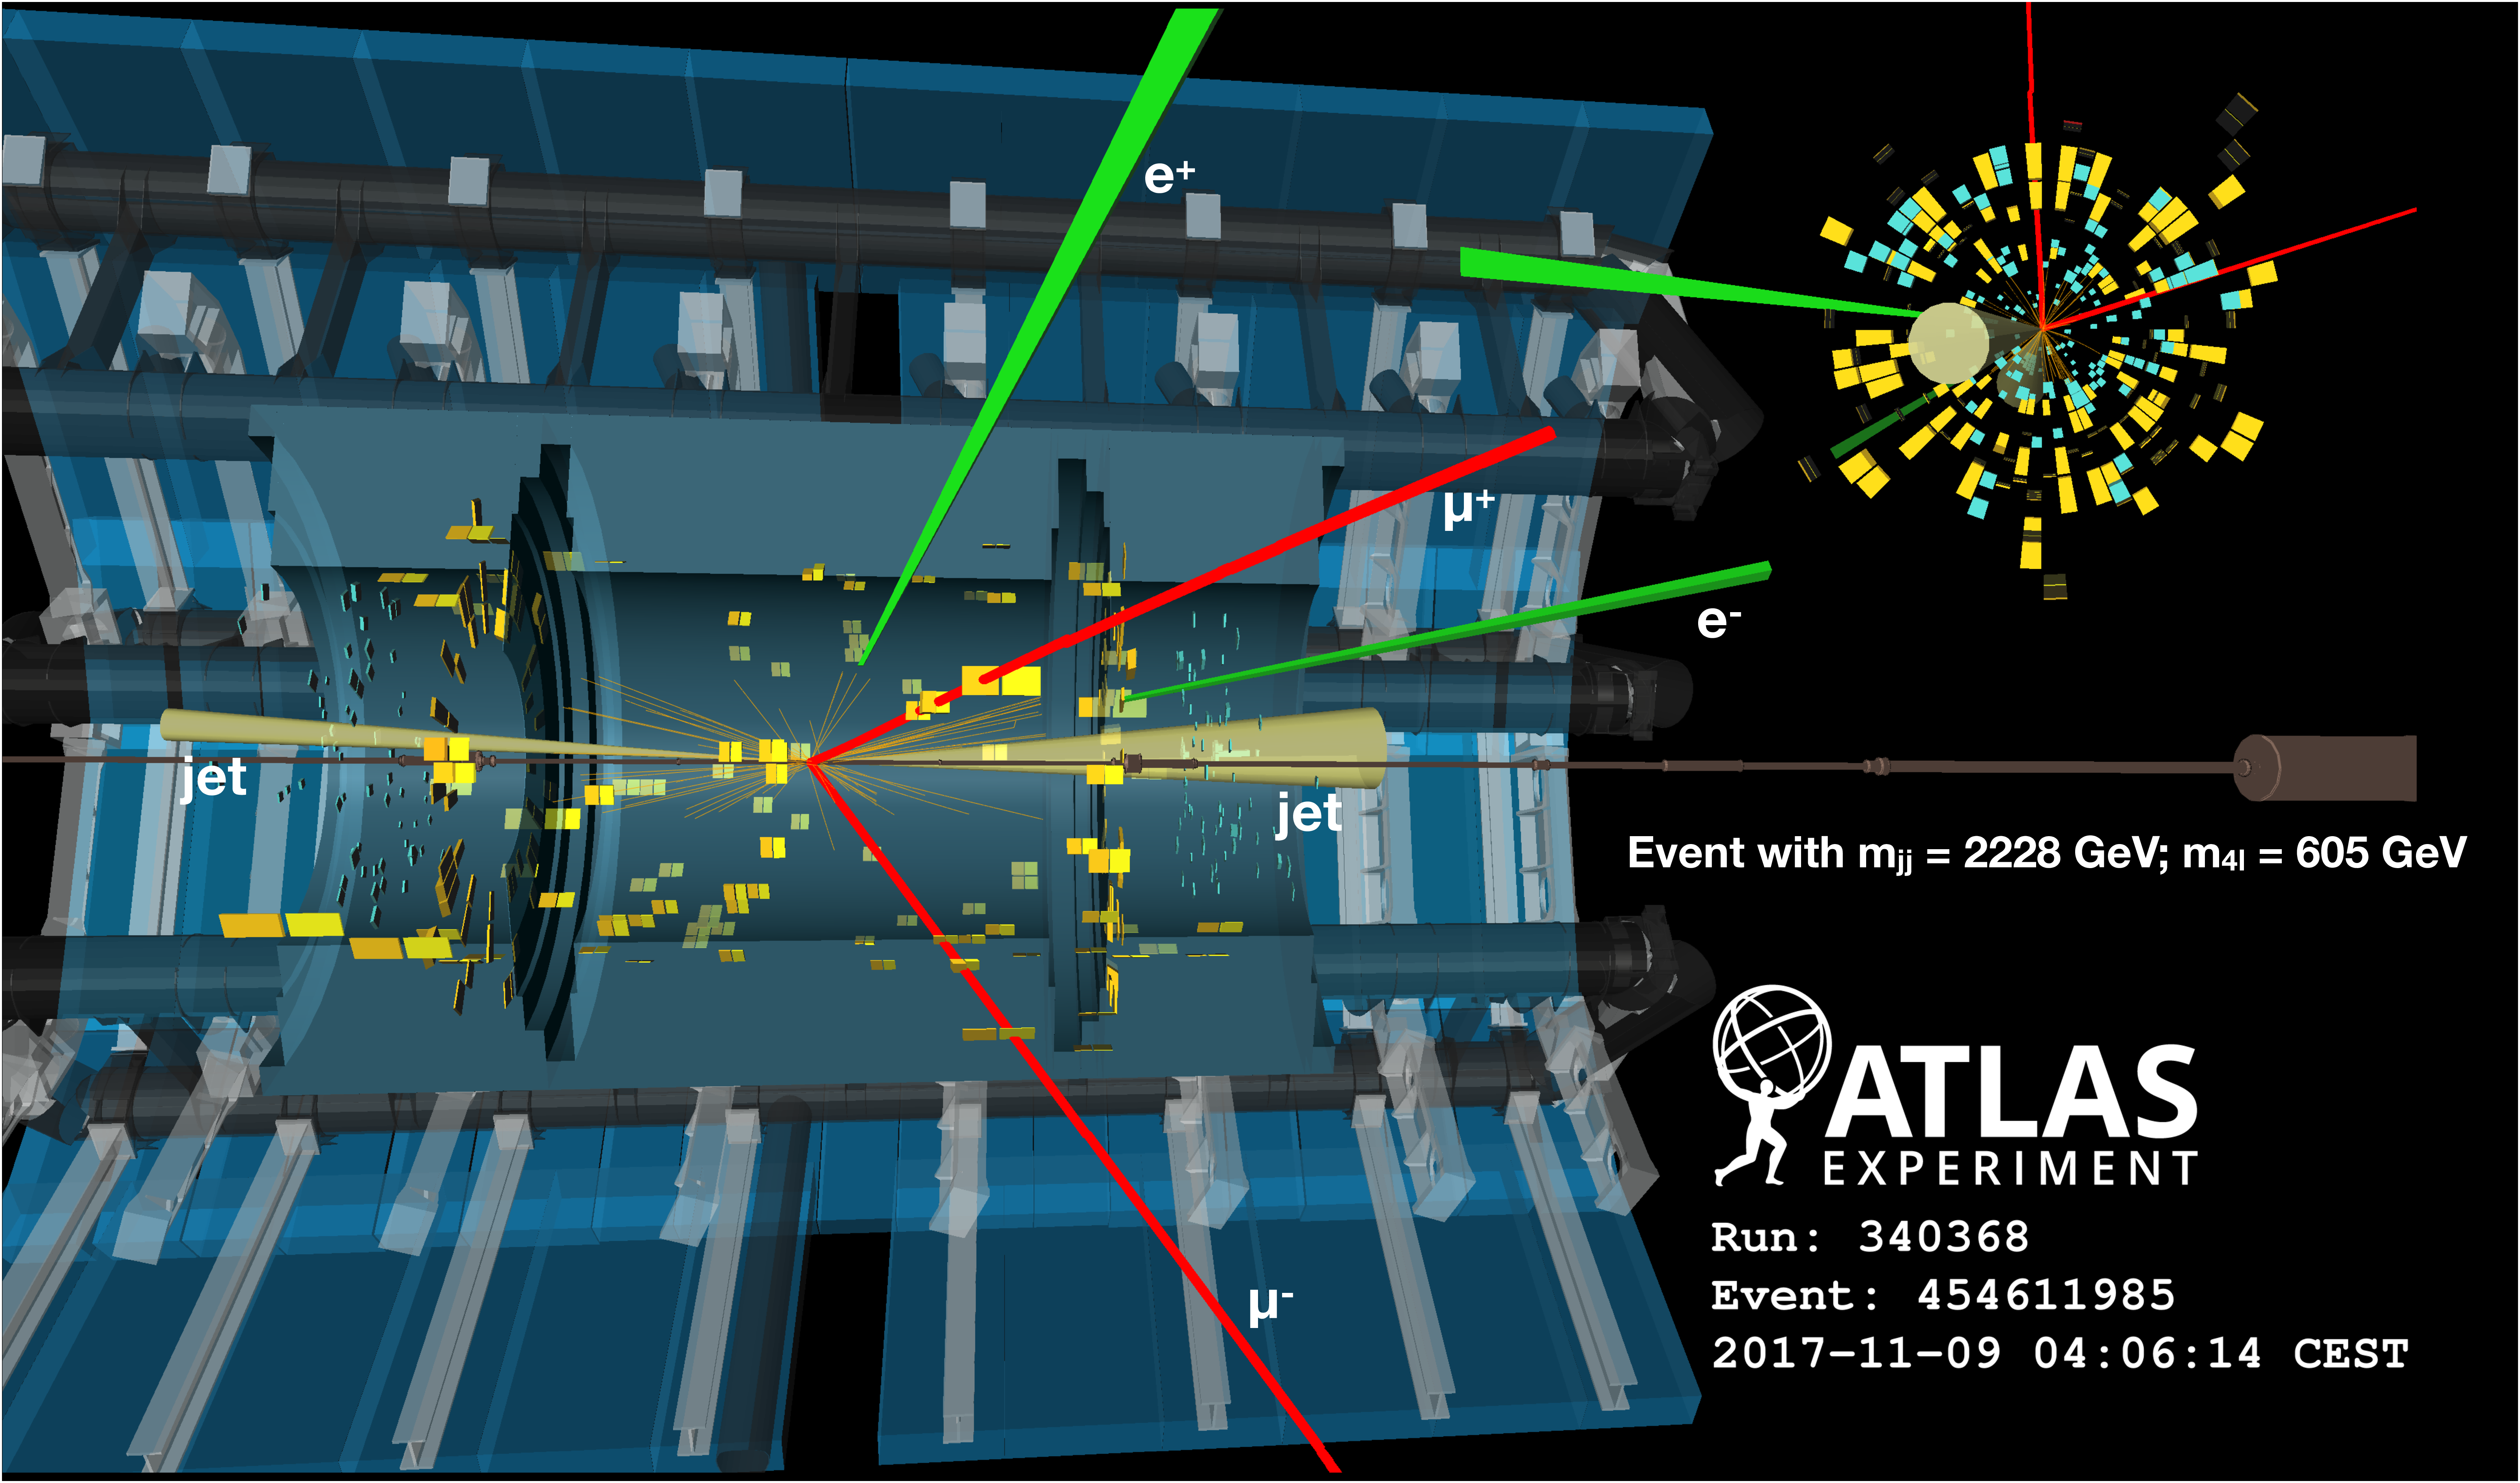
\includegraphics[width=.9\linewidth]{figures/AnalysisOverview/ZZjjEventDisplay.png}  
\caption{Event display of a candidate $pp \rightarrow ZZjj \rightarrow e^+e^-\mu^+\mu^- jj $ recorded by the ATLAS experiment in Run-$2$ $2017$ data-taking period. The invariant mass of the reconstructed four leptons is $m_{4\ell} = 605$ GeV, and that of the reconstructed di-jet is $m_{jj} = 2228$ GeV. The large rapidity separation between the two jet cones (light yellow) on the opposite sides of the ATLAS detector and centrally produced two $Z$ bosons defines the characteristic feature of the EWK production of ZZjj \label{fig:EventDisplayZZjj} \cite{ATLASZZjj}.}
\end{figure}